% Drawing 117/02-1 -- folder 117, batch 02, archive page 24 (PDF page 25).
% Transcription: à gauche de ce carré, un croquis en perspective de l'escalier précédent : un réseau de flèches dont les sommets $e$ sont cerclés, $X$ et $Y$ en bas à gauche, traversé par un trait épais en escalier et par un axe vertical ; on ne le redessine pas.
% Kind: arrow network in perspective (staircase). Method 2 (schematic redraw from the facsimile). Status: partial.
% Notes: Redrawn on a tight crop with every node placed once: thirteen nodes (eight ringed, five plain junctions), and every arrow drawn between the same node centres, from ring to ring (or stopping short of a plain junction); on the page the arrows are shorter strokes in the gaps between the nodes, they are lengthened here to join the nodes they link. Rings carry e where it is written (five), a point in the ring at the back top, X beside the ringed vertex at the lower left; the ringed vertex below it (Y according to the transcription) and the one above X carry no legible letter and are left unlabelled. Arrows: leftward along the four rows (the one into the e at the left heavy), downward along the columns, and the four front-back diagonals. The thick stair-shaped stroke: from the back ring down to the junction where the upper row arrows start, and from the top down, across to the junction on the vertical axis, down to the ring at the right; a second heavy stroke runs down parallel to the axis. The vertical axis (pencil) passes through that junction; the thin pencil diagonal joins the two plain junctions it links. The strokes at the top (two long horizontals, short strokes at the upper right) are drawn as seen, without interpretation. The transcription chose not to redraw this sketch; it is redrawn here as on the page. Redrawn 2026-11-09 (issue 128): to check again.
% Coordinates: 1 unit = 1 mm = 1/100 of the crop width (bbox in page fractions: [0.24, 0.49, 0.44, 0.635]).
% Redrawn by Claude (claude-opus-5-5), issue #73, 2026-11-09; not checked by a human; not compiled (no TeX in the session).
% Rights: reproduces part of the work -- behind RENDER_TRANSCRIPTS, never published by itself.
\documentclass[tikz,border=3pt]{standalone}
\usepackage{amsmath,amssymb}
\usetikzlibrary{patterns,arrows.meta}
\tikzset{pencil/.style={black!45}, struck/.style={black!35}, mark/.style={circle,draw,inner sep=1.3pt}, pt/.style={circle,fill,inner sep=0.9pt}, opt/.style={circle,draw,fill=white,inner sep=1.1pt}}
\begin{document}
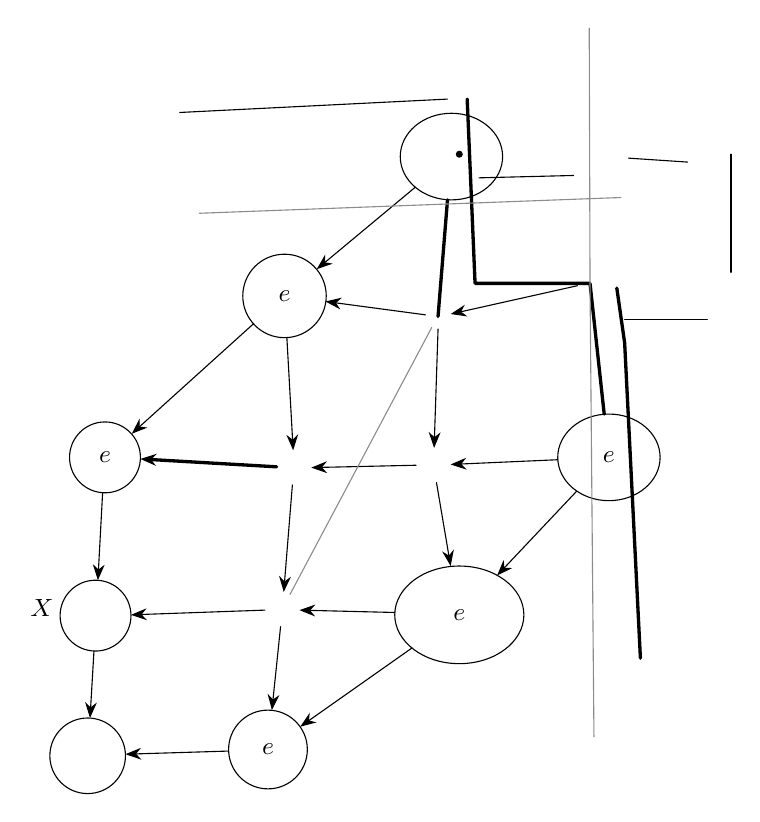
\begin{tikzpicture}[x=1mm,y=1mm,line cap=round,line join=round,font=\scriptsize]
\draw (58.5,-16.3) ellipse[x radius=6.5, y radius=5.5];
\draw (37.3,-34) ellipse[x radius=5.3, y radius=5.3];
\draw (14.5,-54.5) ellipse[x radius=4.5, y radius=4.5];
\draw (78.5,-54.5) ellipse[x radius=6.5, y radius=5.5];
\draw (13.3,-74.6) ellipse[x radius=4.5, y radius=4.5];
\draw (59.5,-74.5) ellipse[x radius=8.2, y radius=6.2];
\draw (12.3,-92.4) ellipse[x radius=4.8, y radius=4.8];
\draw (35.2,-91.6) ellipse[x radius=5, y radius=5];
\node[inner sep=1pt] at (37.3,-34) {\small $e$};
\node[inner sep=1pt] at (14.5,-54.5) {\small $e$};
\node[inner sep=1pt] at (78.5,-54.5) {\small $e$};
\node[inner sep=1pt] at (59.5,-74.5) {\small $e$};
\node[inner sep=1pt] at (35.2,-91.6) {\small $e$};
\node[inner sep=1pt] at (6.5,-73.6) {\small $X$};
\node[pt] at (59.5,-16) {};
\draw[-{Stealth[length=2mm]}] (55.2,-36.4) -- (42.5,-34.7);
\draw[-{Stealth[length=2mm]}] (74.5,-32.7) -- (58.4,-36.3);
\draw[-{Stealth[length=2mm]}] (54,-55.5) -- (40.7,-55.8);
\draw[-{Stealth[length=2mm]}] (72,-54.8) -- (58.4,-55.4);
\draw[-{Stealth[length=2mm]}] (34.8,-73.9) -- (17.8,-74.5);
\draw[-{Stealth[length=2mm]}] (51.3,-74.2) -- (39.2,-73.9);
\draw[-{Stealth[length=2mm]}] (30.2,-91.8) -- (17.1,-92.2);
\draw[-{Stealth[length=2mm]}] (37.6,-39.3) -- (38.4,-53.6);
\draw[-{Stealth[length=2mm]}] (56.8,-38.2) -- (56.3,-53.3);
\draw[-{Stealth[length=2mm]}] (38.3,-58) -- (37.2,-71.6);
\draw[-{Stealth[length=2mm]}] (56.6,-57.7) -- (58.4,-68.3);
\draw[-{Stealth[length=2mm]}] (14.2,-59) -- (13.6,-70.1);
\draw[-{Stealth[length=2mm]}] (13.1,-79.1) -- (12.6,-87.6);
\draw[-{Stealth[length=2mm]}] (36.8,-76) -- (35.7,-86.6);
\draw[-{Stealth[length=2mm]}] (53.9,-20.2) -- (41.4,-30.6);
\draw[-{Stealth[length=2mm]}] (33.4,-37.5) -- (17.9,-51.5);
\draw[-{Stealth[length=2mm]}] (74.4,-58.8) -- (64.3,-69.5);
\draw[-{Stealth[length=2mm]}] (53.5,-78.7) -- (39.3,-88.7);
\draw[very thick,-{Stealth[length=2mm]}] (36.3,-55.7) -- (19,-54.7);
\draw (91,-37) -- (80.5,-37);
\draw[very thick] (58,-21.8) -- (56.8,-36.6);
\draw[very thick] (60.5,-9) -- (61.5,-32.4) -- (76.1,-32.4) -- (77.9,-49);
\draw[very thick] (79.5,-33) -- (80.5,-40) -- (82.5,-80);
\draw[pencil] (76,-0) -- (76.1,-32.4) -- (76.6,-90);
\draw[pencil] (38,-71.9) -- (56,-38);
\draw (24,-10.7) -- (58,-9);
\draw[pencil] (26.5,-23.5) -- (80,-21.5);
\draw (62,-19) -- (74,-18.7);
\draw (81,-16.5) -- (88.5,-17);
\draw (94,-16) -- (94,-31);
\end{tikzpicture}
\end{document}
